\documentclass[12pt]{article}
\usepackage[utf8]{inputenc}
\usepackage[spanish]{babel}
\usepackage{bbding}
\decimalpoint
\usepackage[spanish]{babel}
\usepackage{amsmath}
\usepackage{amsthm}
\usepackage{amssymb}
\usepackage{graphicx}
\usepackage[margin=0.9in]{geometry}
\usepackage{fancyhdr}
\usepackage[inline]{enumitem}
\usepackage{float}
\usepackage{cancel}
\usepackage{minted}
\usepackage{bigints}
\usepackage{color}
\usepackage{xcolor}
\usepackage{subfig}
\usepackage{listingsutf8}
\usepackage{algorithm}
\usepackage{tocloft}
\usepackage[none]{hyphenat}
\usepackage{graphicx}
\usepackage{grffile}
\usepackage{tabularx}
\usepackage[nottoc,notlot,notlof]{tocbibind}
\usepackage{times}
\usepackage{color}
\definecolor{gray97}{gray}{.97}
\definecolor{gray75}{gray}{.75}
\definecolor{gray45}{gray}{.45}
\renewcommand{\cftsecleader}{\cftdotfill{\cftdotsep}}
\pagestyle{fancy}
\setlength{\headheight}{15pt} 
\lhead{Práctica 5: Administrador de procesos en Linux y Windows (2)}
\rhead{\thepage}
\lfoot{ESCOM-IPN}
\renewcommand{\footrulewidth}{0.5pt}
\setlength{\parskip}{0.5em}
\newcommand{\ve}[1]{\overrightarrow{#1}}
\newcommand{\abs}[1]{\left\lvert #1 \right\lvert}
\date{26 de febrero de 2017}
\title{Instalación de Netbeans}
\author{Reporte 1}

\definecolor{pblue}{rgb}{0.13,0.13,1}
\definecolor{pgreen}{rgb}{0,0.5,0}
\definecolor{pred}{rgb}{0.9,0,0}
\definecolor{pgrey}{rgb}{0.46,0.45,0.48}
\lstset{tabsize=1}

\usepackage{listings}
\lstset{ frame=Ltb,
framerule=0pt,
aboveskip=0.5cm,
framextopmargin=3pt,
framexbottommargin=3pt,
framexleftmargin=0.4cm,
framesep=0pt,
rulesep=.4pt,
backgroundcolor=\color{gray97},
rulesepcolor=\color{black},
%
stringstyle=\ttfamily,
showstringspaces = false,
basicstyle=\small\ttfamily,
commentstyle=\color{gray45},
keywordstyle=\bfseries,
%
numbers=left,
numbersep=15pt,
numberstyle=\tiny,
numberfirstline = false,
breaklines=true,
}

% minimizar fragmentado de listados
\lstnewenvironment{listing}[1][]
{\lstset{#1}\pagebreak[0]}{\pagebreak[0]}

\lstdefinestyle{consola}
{basicstyle=\scriptsize\bf\ttfamily,
backgroundcolor=\color{gray75},
}

\lstdefinestyle{C}
{language=C,
}
 \lstset{style=CompilandoStyle}                                  %Use this style

    \usepackage{minted} % Paquete que permite citar codigo
    \usemintedstyle{borland} % Aqui se define el colorscheme para minted
    \setminted{
        fontsize = \scriptsize, % Ajusta el codigo a la hoja
        baselinestretch = 1,
        linenos, % set numbers
        breaklines=true, % Hace un salto de linea automatico en caso de que se llege al final de la line
        tabsize=3 
    }
%%%%%%%%%%%%%%%%%%%%%

\lstdefinestyle{customc}{
  belowcaptionskip=1\baselineskip,
  breaklines=true,
  frame=L,
  xleftmargin=\parindent,
  language=C,
  showstringspaces=false,
  basicstyle=\footnotesize\ttfamily,
  keywordstyle=\bfseries\color{green!40!black},
  commentstyle=\itshape\color{purple!40!black},
  identifierstyle=\color{blue},
  stringstyle=\color{orange},
}

\lstdefinestyle{customasm}{
  belowcaptionskip=1\baselineskip,
  frame=L,
  xleftmargin=\parindent,
  language=[x86masm]Assembler,
  basicstyle=\footnotesize\ttfamily,
  commentstyle=\itshape\color{purple!40!black},
}

\lstset{escapechar=@,style=customc}

    % =====  CODE EDITOR =========
    \lstdefinestyle{CompilandoStyle} {                              %This is Code Style
        backgroundcolor=\color{BlueGrey800MD},                      %Background Color  
        basicstyle=\tiny\color{white},                              %Font color
        commentstyle=\color{BlueGrey100MD},                         %Comment color
        stringstyle=\color{TealMD},                                 %String color
        keywordstyle=\color{Green100MD},                            %keywords color
        numberstyle=\tiny\color{TealMD},                            %Size of a number
        frame=shadowbox,                                            %Adds a frame around the code
        breakatwhitespace=true,                                     %Style                       
        breaklines=true,                                            %Style                   
        keepspaces=true,                                            %Style                   
        numbers=left,                                               %Style                   
        numbersep=10pt,                                             %Style 
        xleftmargin=\parindent,                                     %Style 
        tabsize=4                                                   %Style 
    }
 
    \lstset{style=CompilandoStyle}                                  %Use this style

    \usepackage{minted} % Paquete que permite citar codigo
    \usemintedstyle{borland} % Aqui se define el colorscheme para minted
    \setminted{
        fontsize = \scriptsize, % Ajusta el codigo a la hoja
        baselinestretch = 1,
        linenos, % set numbers
        breaklines=true, % Hace un salto de linea automatico en caso de que se llege al final de la line
        tabsize=3 
    }


%Permite crear columnas en el documento
\usepackage{multicol} 
\usepackage{color}
\usepackage{comment}
\newcommand{\tabitem}{~~\llap{\textbullet}~~}
\newcommand{\subtabitem}{~~~~\llap{\textbullet}~~}


\bibliographystyle{IEEEtran}
\begin{document}
		\begin{titlepage}
			\begin{center}
				
				% Upper part of the page. The '~' is needed because \\
				% only works if a paragraph has started.
				
				\noindent
				\begin{minipage}{0.5\textwidth}
					\begin{flushleft} \large
						\includegraphics[width=0.3\textwidth]{../ipn.png}
					\end{flushleft}
				\end{minipage}%
				\begin{minipage}{0.55\textwidth}
					\begin{flushright} \large
						\includegraphics[width=0.7\textwidth]{../escom.png}
					\end{flushright}
				\end{minipage}
				
				\textsc{\LARGE Instituto Politécnico Nacional}\\[0.5cm]
				
				\textsc{\Large Escuela Superior de Cómputo}\\[1cm]
				
				% Title
				
				{ \huge Práctica 5 - Administrador de procesos en Linux y Windows (2) \\[1cm] }
				
				{ \Large Unidad de aprendizaje: Sistemas Operativos} \\[1cm]
				
				{ \Large Grupo: 2CM8 } \\[1cm]
				
				\noindent
				\begin{minipage}{0.5\textwidth}
					\begin{flushleft} \large
						\emph{Alumnos(a):}\\
						
						\begin{tabular}{ll}
						 Briones Tapia Mariana \\
						 Méndez Mejía Sergio Ernesto \\
					     Nicolás Sayago Abigail\\
					     Ramos Diaz Enrique \\
					     
					\end{tabular}
					\end{flushleft}
				\end{minipage}%
				\begin{minipage}{0.5\textwidth}
					\begin{flushright} \large
						\emph{Profesor(a):} \\
						Cortes Galicia Jorge  \\
					\end{flushright}
				\end{minipage}
				
				\vfill
				
				% Bottom of the page
				{\large 29 de septiembre 2018}
			\end{center}
		\end{titlepage}
	
	\tableofcontents
	\newpage
	
	
% //////////////////////////////////////////////////////////////////////////////////////////////////////////////
%                                                   COMPETENCIAS
% /////////////////////////////////////////////////////////////////////////////////////////////////////////////

	\section{Competencias}
        El alumno aprende a familiarizarse con el administrador de procesos del sistema operativo Linux y Windows a través de la creación de procesos ligeros (hilos) para el desarrollo de aplicaciones concurrentes sencillas.
        
        \begin{itemize}
            \item Revisión de la creación de procesos ligeros (hilos) en Linux y Windows.
            \item Revisión de las llamadas al sistema y funciones de biblioteca para Hilos en ambos sistemas operativos.
            \item Desarrollo de aplicaciones concurrentes usando hilos tanto en Linux como en Windows.
        \end{itemize}
% //////////////////////////////////////////////////////////////////////////////////////////////////////////////
%                                                   DESARROLLO
% /////////////////////////////////////////////////////////////////////////////////////////////////////////////
	
    \section{Desarrollo}
    \subsection{Puntos a observar y reportar}
    
            
            % ///////////////////////////////////////////////////////////////////////////////////////////////
            %                              SECCION DE LINUX
            % ///////////////////////////////////////////////////////////////////////////////////////////////
        
        
        \subsubsection{Sección Linux:}
        Investigación de los siguientes comandos:
        
        \begin{itemize}
            \item[\Checkmark] \textbf{pthread\_create() :}
            La función pthread\_create() inicia un nuevo hilo en la llamada proceso. El nuevo hilo comienza la ejecución invocando start\_routine(); arg se pasa como el único argumento de start\_routine().
            
            El argumento attr apunta a una estructura pthread\_attr\_t cuyo contenido se utilizan en el momento de la creación de hilos para determinar los atributos para el nuevo hilo; esta estructura se inicializa utilizando pthread\_attr\_init(). Si attr es NULL, entonces el hilo se crea con atributos por defecto.

            Antes de regresar, una llamada exitosa a pthread\_create() almacena la ID del nuevo hilo en el búfer apuntado por hilo; este identificador se utiliza para referirse al hilo en llamadas subsiguientes a otras funciones pthreads.
            
            En caso de éxito, pthread\_create() devuelve 0; en caso de error, devuelve un número de error, y los contenidos de * hilo están indefinidos.
            
            \item[\Checkmark] \textbf{pthread\_join() :}
            La función pthread\_join() espera el hilo especificado por un subproceso para terminar. Si ese hilo ya ha terminado, entonces pthread\_join() devuelve inmediatamente el hilo especificado por hilo debe poder unirse.
            
            Si retval no es NULL, pthread\_join() copia el estado de salida de el subproceso de destino (es decir, el valor que el subproceso de destino suministró a pthread\_exit() ) en la ubicación señalada por retval . 
            
            En caso de éxito, pthread\_join() devuelve 0; en caso de error, devuelve un número de error.
            
             \item[\Checkmark] \textbf{pthread\_self() :}
             La función pthread\_self() devuelve el ID del hilo que llama.
             Este es el mismo valor que se devuelve en el hilo * en el pthread\_create() llamada que creó este hilo. Esta función siempre tiene éxito, devolviendo el ID del hilo que llama.
             
             \item[\Checkmark] \textbf{pthread\_exit() :}
             La función pthread\_exit() termina llamada del hilo y devuelve un valor a través de retval que (si el hilo se puede unir) está disponible para otro hilo en el mismo proceso que llama a pthread\_join(). No tiene retorno.
             
             \item[\Checkmark] \textbf{scandir() :}
             La función scandir() escanea el directorio dirp, llamando a filter() en cada entrada de directorio. Las entradas para las que filter() devuelve un valor distinto de cero son almacenados en cadenas asignadas a través de malloc(), ordenados usando qsort (3) con la función de comparación compar() y se recopila en la lista de nombres de matriz que se asigna a través de malloc(). Si el filtro es NULL, todas las entradas son seleccionadas.
             
             La función scandir() devuelve el número de entradas de directorio seleccionadas o -1 si se produce un error.

            Las funciones alphasort() y versionsort() devuelven un número entero menor que, igual o mayor que cero si se considera que el primer argumento es respectivamente menor que, igual o mayor que el segundo
             
             \item[\checkmark] \textbf{stat() :}
             La llamada al sistema stat() devuelve información sobre un archivo. No se requieren permisos del archivo mismo, pero en el caso de stat() y lstat() - permisos de ejecución (de búsqueda) son requeridos en todos los directorios de la ruta que lleva al archivo.
                \begin{itemize}
                    \item stat() recupera información sobre el archivo apuntado por la ruta y esta se guarda en un buffer.

                    \item lstat() es idéntico a stat(), excepto que si la ruta del archivo es un enlace simbólico, entonces devuelve información sobre el enlace en sí, no del archivo al que se refiere

                    \item fstat() es idéntico a stat(), excepto que el archivo sobre el cual se va a recuperar información está especificado por su descriptor.
                \end{itemize}
        
        \end{itemize}
        
        \begin{itemize}
            \item[\Checkmark] \textbf{Punto 2: Creación de un nuevo hilo} 
            \inputminted{c++}{Code/Linux/2.c}
            \newpage
            \item[\Checkmark] \textbf{Punto 3: Creación de hilos} 
            \inputminted{c++}{Code/Linux/3.c}
        \end{itemize}
        
        
            % ///////////////////////////////////////////////////////////////////////////////////////////////
            %                              SECCION DE WINDOWS
            % ///////////////////////////////////////////////////////////////////////////////////////////////
            
        \subsubsection{Sección Windows:}
        \begin{itemize}
            \item[\Checkmark] \textbf{Punto 4: Creación de hilos} 
            \inputminted{c++}{Code/Windows/4.c}
        \end{itemize}

    		
       
        % ////////////////////////////////////////////////////////////////////////////////////////////////////
        % 						CODIGOS FUENTE DE LOS PROGRAMAS DESARROLLADOS
        % ////////////////////////////////////////////////////////////////////////////////////////////////////

    	\subsection{Códigos fuente de los programas desarrollados}
    	
    	\subsubsection{Sección Linux}

    	\begin{itemize}
    	    \item[\Checkmark] \textbf{Programa 5.- Creación de hilos con procesos}
    	        \inputminted{c++}{Code/Linux/5.c}
    	        
    	    \item[\Checkmark] \textbf{Programa 6.- Operaciones con matrices utilizando creación de hilos}
    	    
    	    \textbf{Creación de hilos}
    	    
    	        \inputminted{c++}{Code/Linux/6.c}
    	        
    	    \textbf{Funciones con las operaciones de matrices}
    	    
    	        \inputminted{c++}{Code/Linux/funciones.h}
    	        
    	    \item[\Checkmark] \textbf{Programa 7.- Creación de directorios y copia de archivos concurrente utilizando creación de hilos}
    	        \inputminted{c++}{Code/Linux/7.c}

    	
    	\end{itemize}
    	
    	\subsubsection{Sección Windows}
    	
    	\begin{itemize}
    	    \item[\Checkmark] \textbf{Programa 5.- Creación de hilos con procesos}
    	    
    	        \textbf{Proceso padre}
    	        
    	        \inputminted{c++}{Code/Windows/5_padre.c}
    	        \textbf{Proceso hijo - Creación de hilos}
    	        
 				\inputminted{c++}{Code/Windows/5_hijo.c}
    	        
    	    \item[\Checkmark] \textbf{Programa 6.- Operaciones con matrices utilizando creación de hilos}
    	    
    	        \textbf{Creación de hilos}
    	    
    	        \inputminted{c++}{Code/Windows/6.c}
    	        
    	    \textbf{Funciones con las operaciones de matrices}
    	    
    	        \inputminted{c++}{Code/Windows/funciones.h}
    	        
    	    \item[\Checkmark] \textbf{Programa 7.- Creación de directorios y copia de archivos concurrente utilizando creación de hilos}
    	        \inputminted{c++}{Code/Windows/7.c}

            
    	\end{itemize}
    
        % ////////////////////////////////////////////////////////////////////////////////////////////////////
        %                               PANTALLAS DE EJECUCIÓN DE LOS PROGRAMAS DESARROLLADOS
        % ////////////////////////////////////////////////////////////////////////////////////////////////////
        
        \newpage
    	\subsection{Pantallas de ejecución de los programas desarrollados}
    		
    		% ///////////////////////////////////////////////////////////////////////////////////////////////
	        % 											SECCION LINUX
	        % ///////////////////////////////////////////////////////////////////////////////////////////////
	        
    		\subsubsection{Sección Linux:}
            
    \begin{itemize}
             \item[\Checkmark] \textbf{Programa 2: Creación de un nuevo hilo en Linux}
             \begin{figure}[h!]
			          \centering
			         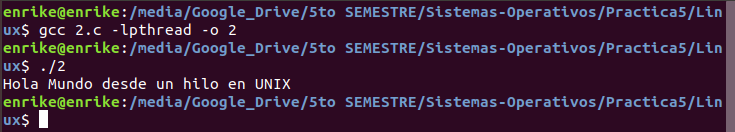
\includegraphics[width=0.9\textwidth]{Practica5/Images/linux/2.png}
			         \end{figure}
              \item[\Checkmark] \textbf{Programa 3: Creación de hilos en Linux}
              \begin{figure}[h!]
			          \centering
			         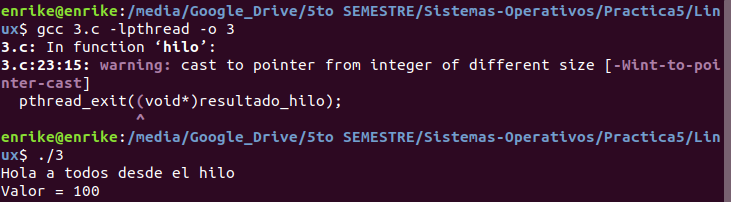
\includegraphics[width=0.9\textwidth]{Practica5/Images/linux/3.png}
			         \end{figure}
             
    
			 \item[\Checkmark] \textbf{Programa 5.- Creación de hilos con procesos}
			 
    	       \begin{figure}[h!]
			          \centering
			         \subfloat{\includegraphics[width=0.58\textwidth]{Practica5/Images/linux/5_1.png}}
                     \subfloat{\includegraphics[width=0.52\textwidth]{Practica5/Images/linux/5_2.png}}
			         \end{figure}
			         \newpage
			          \begin{figure}[h!]
			          \centering
			         \subfloat{\includegraphics[width=0.54\textwidth]{Practica5/Images/linux/5_3.png}}
                     \subfloat{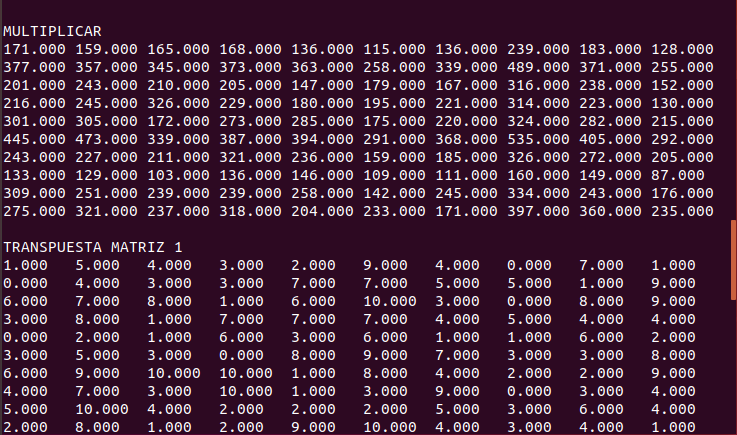
\includegraphics[width=0.54\textwidth]{Practica5/Images/linux/5_4.png}}
			         \end{figure}
			         
			          \begin{figure}[h!]
			          \centering
			         \subfloat{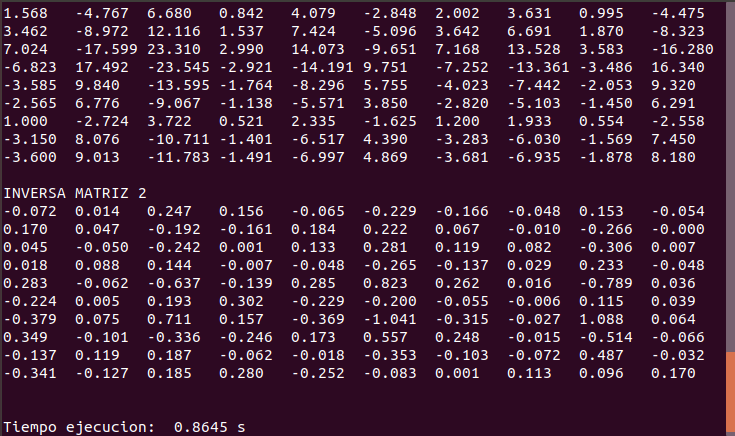
\includegraphics[width=0.54\textwidth]{Practica5/Images/linux/5_5.png}}
                     \subfloat{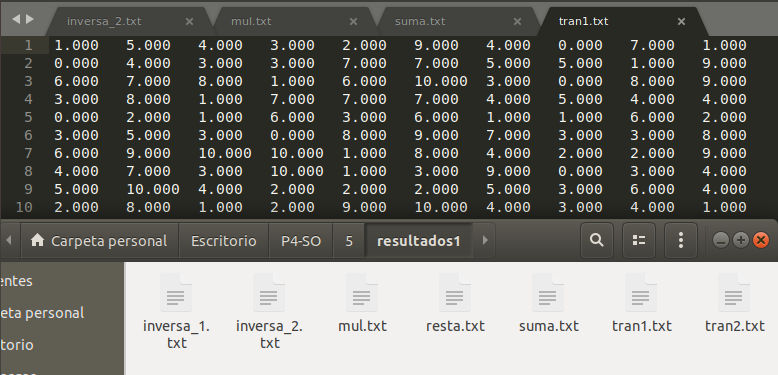
\includegraphics[width=0.54\textwidth]{Practica5/Images/linux/5_6.png}}
			         \end{figure}
			         
			         \newpage
			        \begin{figure}[h!]
			          \centering
			         \subfloat{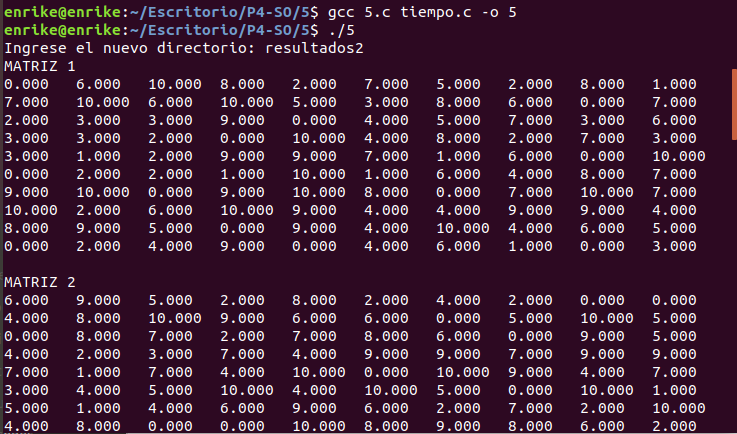
\includegraphics[width=0.54\textwidth]{Practica5/Images/linux/5_7.png}}
                     \subfloat{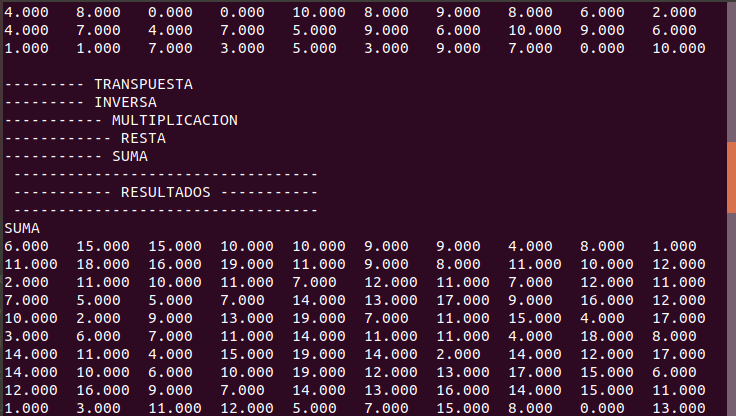
\includegraphics[width=0.54\textwidth]{Practica5/Images/linux/5_8.png}}
			         \end{figure}
			         
			          \begin{figure}[h!]
			          \centering
			         \subfloat{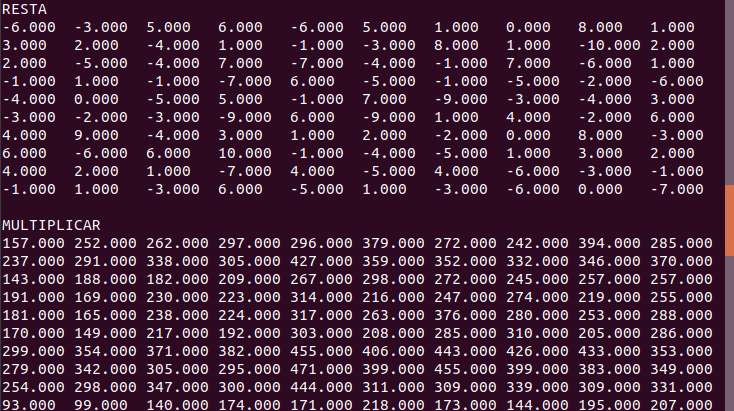
\includegraphics[width=0.54\textwidth]{Practica5/Images/linux/5_9.png}}
                     \subfloat{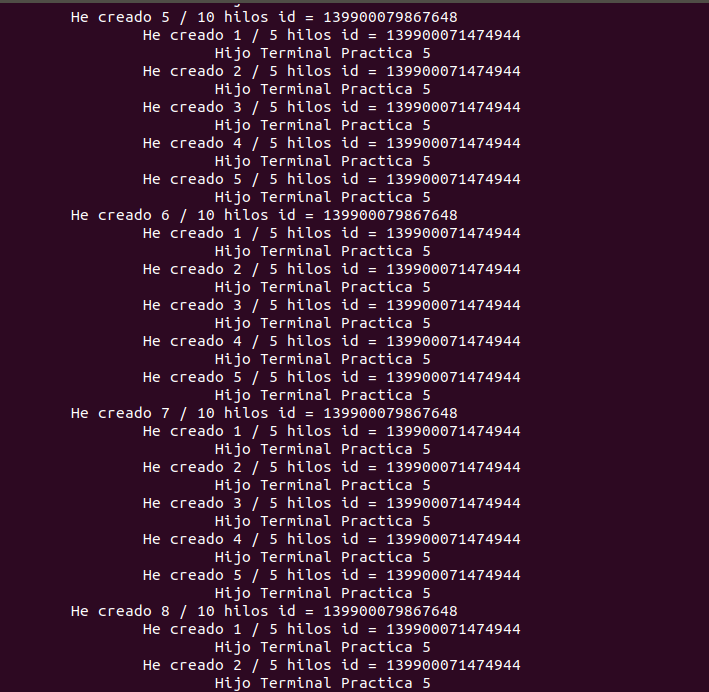
\includegraphics[width=0.54\textwidth]{Practica5/Images/linux/5_10.png}}
			         \end{figure}
			         \begin{figure}[h!]
			          \centering
			         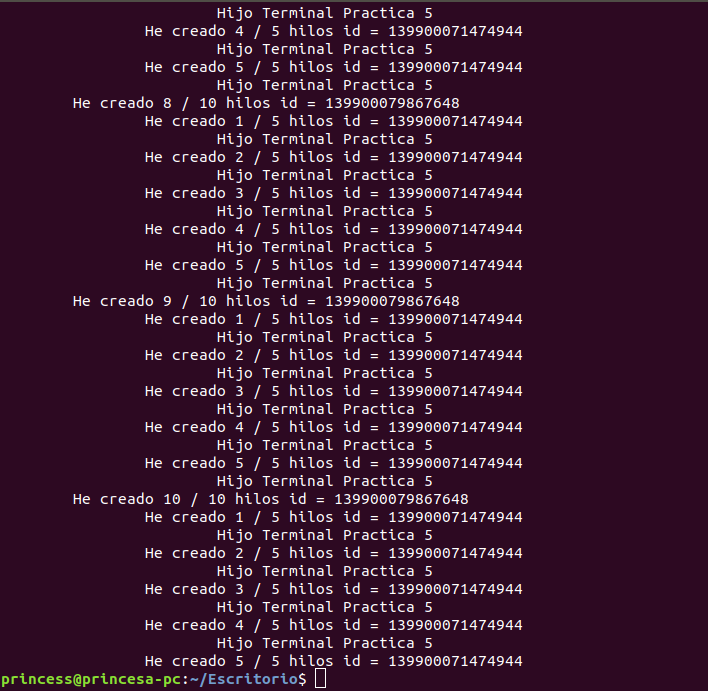
\includegraphics[width=0.54\textwidth]{Practica5/Images/linux/5_11.png}
			         \end{figure}
    	        \newpage
    	    \item[\Checkmark] \textbf{Programa 6.- Operaciones con matrices utilizando creación de hilos}
    	    
    	        \begin{figure}[h!]
			          \centering
			         \subfloat{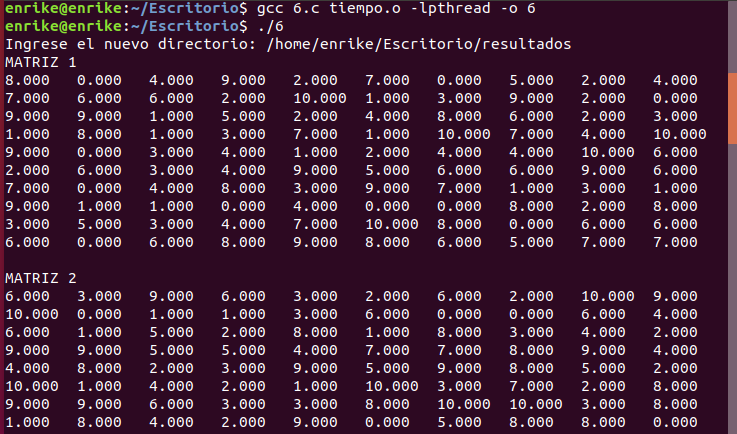
\includegraphics[width=0.55\textwidth]{Practica5/Images/linux/6_1.png}}
                     \subfloat{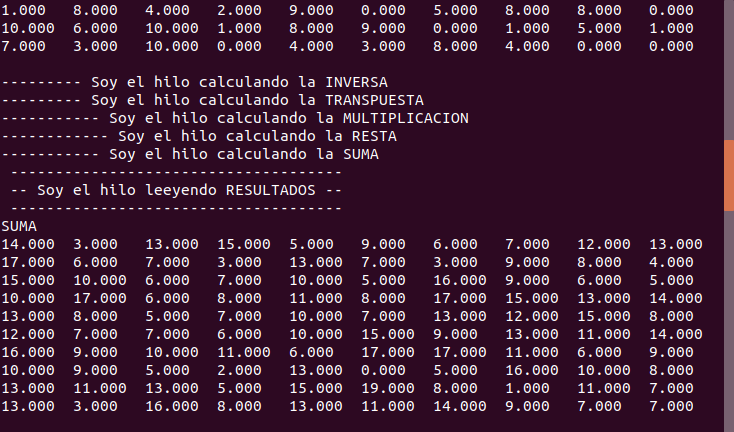
\includegraphics[width=0.55\textwidth]{Practica5/Images/linux/6_2.png}}
			         \end{figure}

			     \begin{figure}[h!]
			          \centering
			         \subfloat{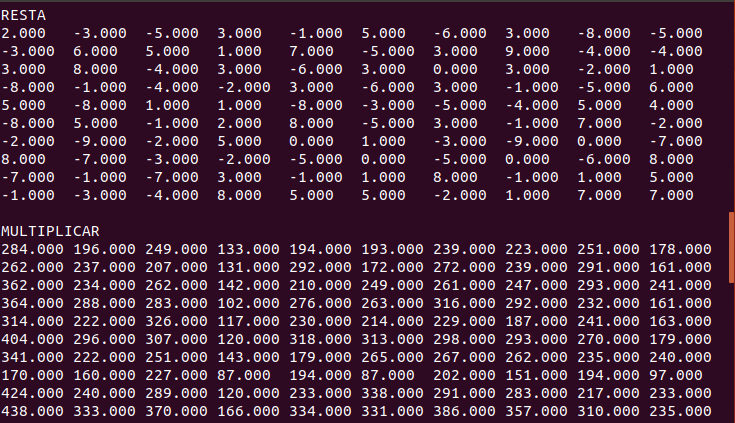
\includegraphics[width=0.55\textwidth]{Practica5/Images/linux/6_3.png}}
                     \subfloat{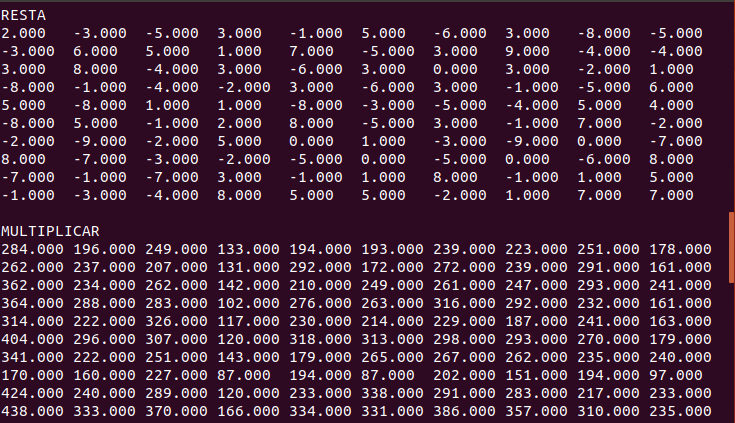
\includegraphics[width=0.55\textwidth]{Practica5/Images/linux/6_3.png}}
			         \end{figure}
			         
			         \newpage
			         \begin{figure}[h!]
			          \centering
			         \subfloat{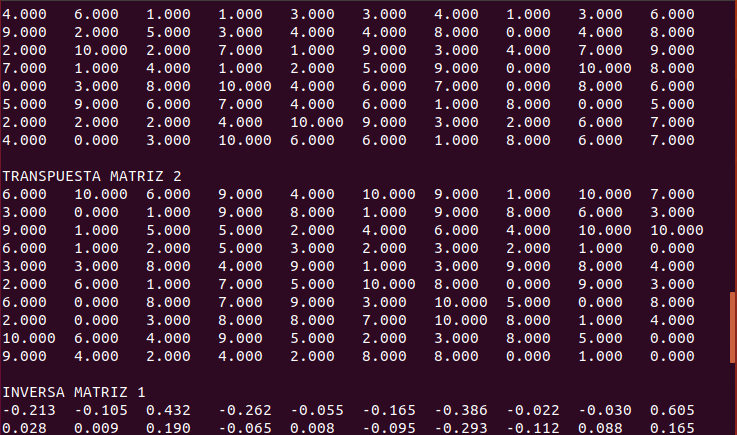
\includegraphics[width=0.55\textwidth]{Practica5/Images/linux/6_4.png}}
                     \subfloat{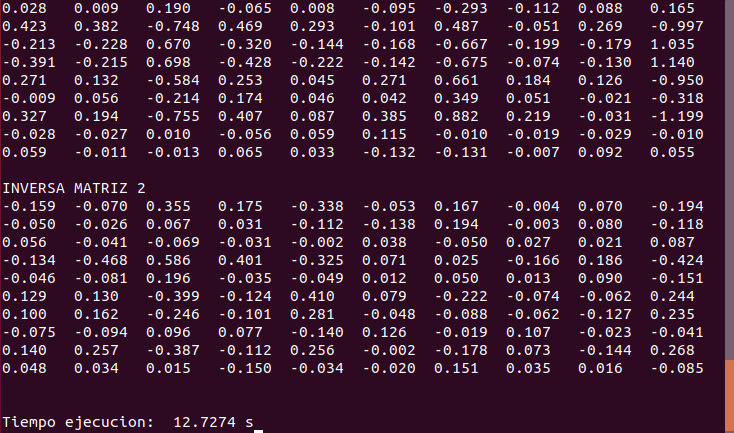
\includegraphics[width=0.55\textwidth]{Practica5/Images/linux/6_5.png}}
			         \end{figure}
			         
			         \begin{figure}[h!]
			          \centering
			         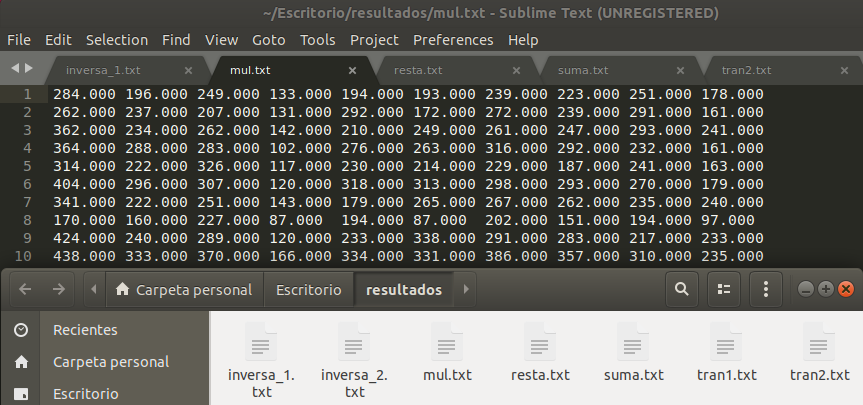
\includegraphics[width=0.82\textwidth]{Practica5/Images/linux/6_6.png}
			         \end{figure}
    	        
    	    \item[\Checkmark] \textbf{Programa 7.- Creación de directorios y copia de archivos concurrente utilizando creación de hilos}
    	    
    	        \begin{figure}[h!]
			          \centering
			         \includegraphics[width=0.82\textwidth]{Practica5/Images/linux/7_3.png}
                    \end{figure}
			         
			         \begin{figure}[h!]
			          \centering \includegraphics[width=0.82\textwidth]{Practica5/Images/linux/7_4.png}
			         \end{figure}
			         
			         \begin{figure}[h!]
			          \centering 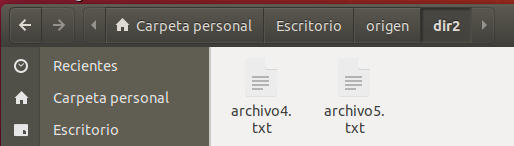
\includegraphics[width=0.72\textwidth]{Practica5/Images/linux/7_6.png}
			         \end{figure}
			         
			         \begin{figure}[h!]
			          \centering 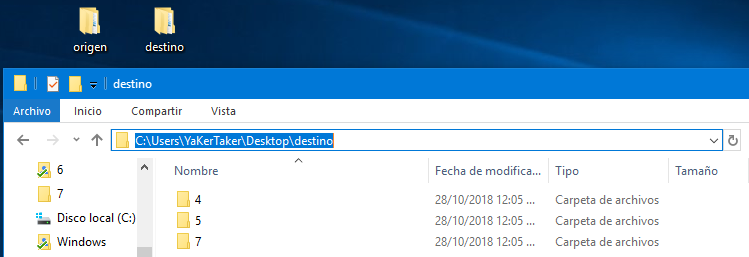
\includegraphics[width=0.72\textwidth]{Practica5/Images/linux/7_7.png}
			         \end{figure}
			         
			         \begin{figure}[h!]
			          \centering \includegraphics[width=0.85\textwidth]{Practica5/Images/linux/7_1.png}
                     
\includegraphics[width=0.85\textwidth]{Practica5/Images/linux/7_2.png}
			         \end{figure}
			         
			         \begin{figure}[h!]
			          \centering 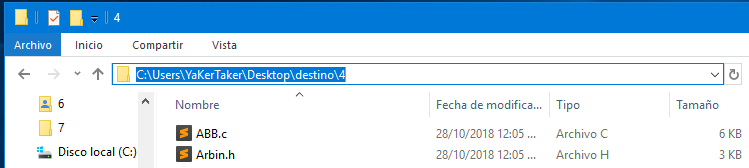
\includegraphics[width=0.72\textwidth]{Practica5/Images/linux/7_8.png}
			         \end{figure}
			         
			         \begin{figure}[h!]
			          \centering 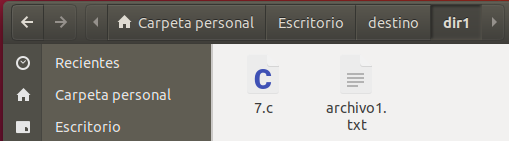
\includegraphics[width=0.7\textwidth]{Practica5/Images/linux/7_9.png}
			         \end{figure}
			         
			         \begin{figure}[h!]
			          \centering 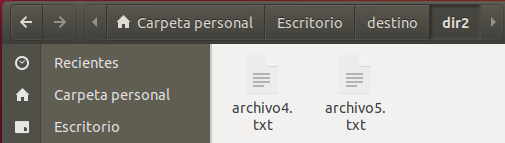
\includegraphics[width=0.7\textwidth]{Practica5/Images/linux/7_10.png}
			         \end{figure}
			         \begin{figure}[h!]
			          \centering 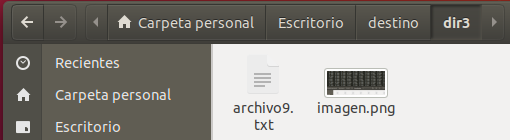
\includegraphics[width=0.7\textwidth]{Practica5/Images/linux/7_11.png}
			         \end{figure}
			         
			         \begin{figure}[h!]
			          \centering 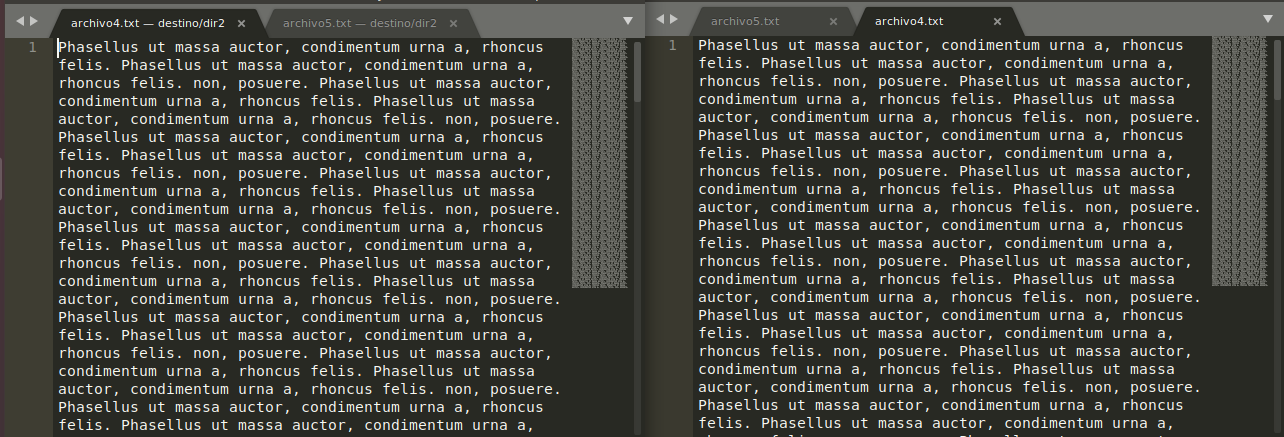
\includegraphics[width=0.9\textwidth]{Practica5/Images/linux/7_12.png}
			         \end{figure}
			         
			         \begin{figure}[h!]
			          \centering 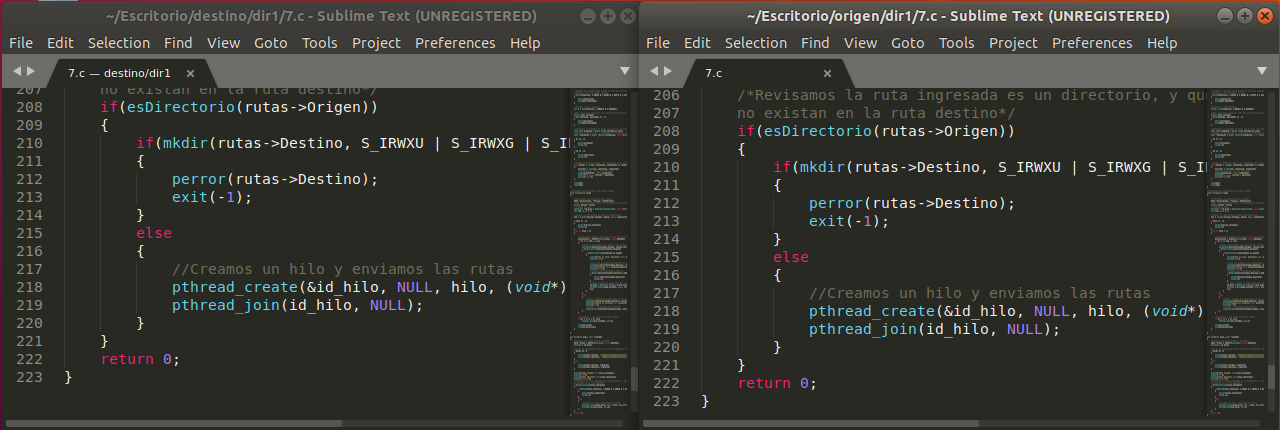
\includegraphics[width=0.9\textwidth]{Practica5/Images/linux/7_13.png}
			         \end{figure}
	
	\end{itemize}		 
			 
			 
			% ///////////////////////////////////////////////////////////////////////////////////////////////
	        % 											SECCION WINDOWS
	        % ///////////////////////////////////////////////////////////////////////////////////////////////	    
	        
\newpage
		    \subsubsection{Sección Windows:}
		    
    		    \begin{itemize}

            \item[\Checkmark] \textbf{Programa 4: Creación de hilos en Windows}
            \begin{figure}[h!]
			          \centering
			         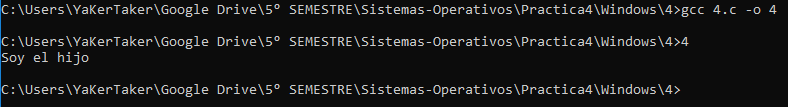
\includegraphics[width=0.9\textwidth]{Practica5/Images/windows/4.PNG}
			         \end{figure} 
            
			 \item[\Checkmark] \textbf{Programa 5.- Creación de hilos con procesos}
			 
    	       \begin{figure}[h!]
			          \centering
			         \includegraphics[width=0.9\textwidth]{Practica5/Images/windows/5_1.png}
			         \end{figure} 
\begin{figure}[h!]
			          \centering
			         \includegraphics[width=0.9\textwidth]{Practica5/Images/windows/5_2.png}
			         \end{figure} 
\begin{figure}[h!]
			          \centering
			         \includegraphics[width=\textwidth]{Practica5/Images/windows/5_3.png}
			         \end{figure}
    	        
    	   
 \item[\Checkmark] \textbf{Programa 6.- Operaciones con matrices utilizando creación de hilos}
    	    
    	        \begin{figure}[h!]
			          \centering
			         \subfloat{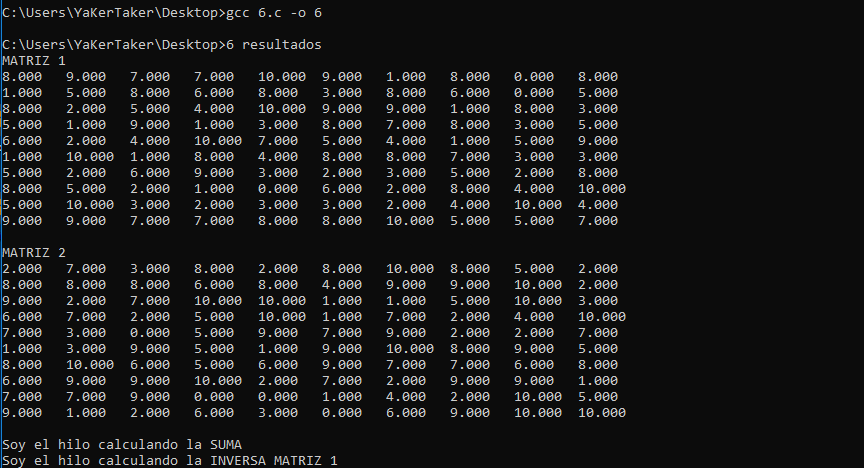
\includegraphics[width=0.56\textwidth]{Practica5/Images/windows/6_1.PNG}}
                     \subfloat{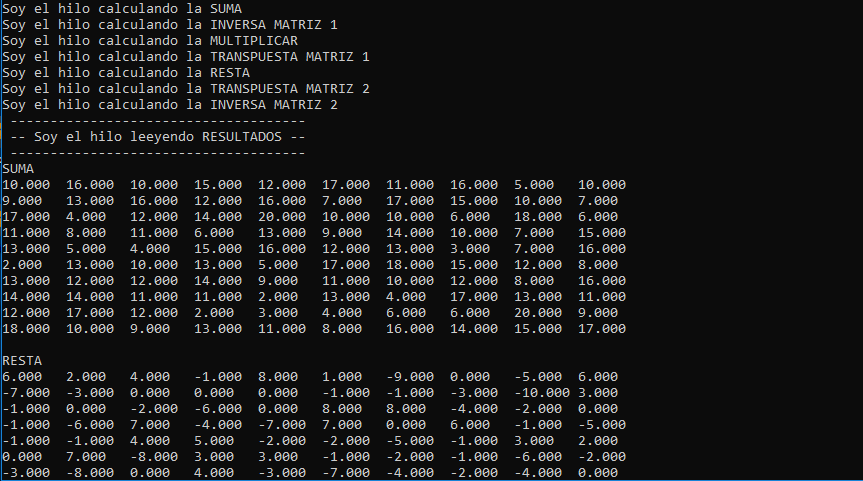
\includegraphics[width=0.55\textwidth]{Practica5/Images/windows/6_2.PNG}}
			         \end{figure}
			         
			         \begin{figure}[h!]
			          \centering
			         \subfloat{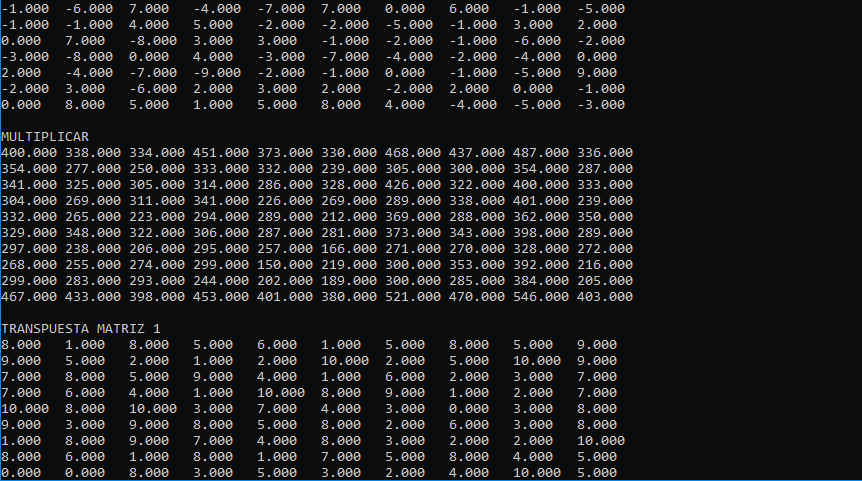
\includegraphics[width=0.56\textwidth]{Practica5/Images/windows/6_3.PNG}}
                     \subfloat{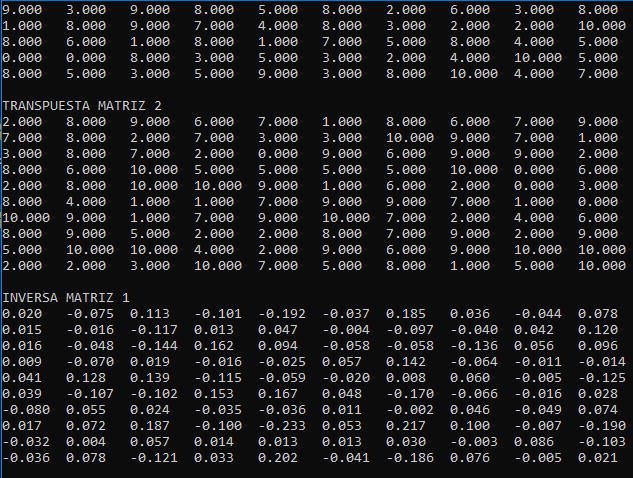
\includegraphics[width=0.55\textwidth]{Practica5/Images/windows/6_4.PNG}}
			         \end{figure}
			         
			         \begin{figure}[h!]
			          \centering
			         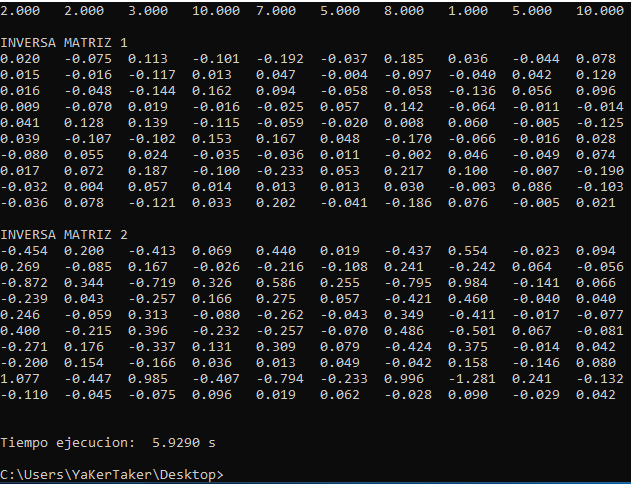
\includegraphics[width=0.65\textwidth]{Practica5/Images/windows/6_5.PNG}
                     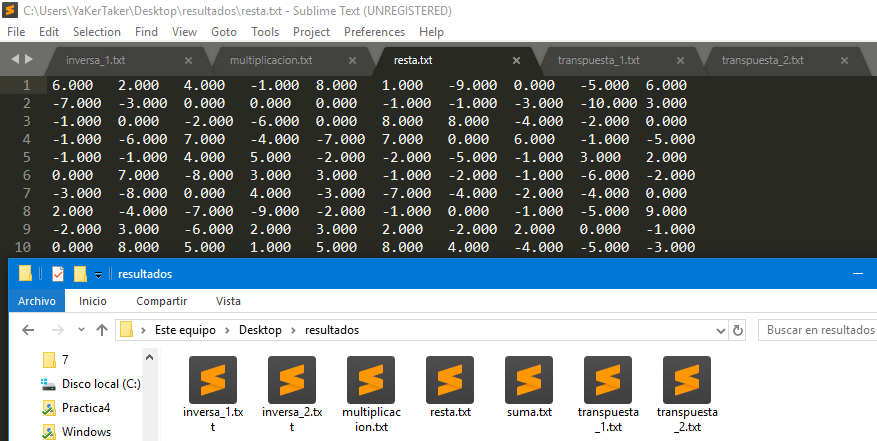
\includegraphics[width=0.65\textwidth]{Practica5/Images/windows/6_6.PNG}
			         \end{figure}
    	        \newpage
    	    \item[\Checkmark] \textbf{Programa 7.- Creación de directorios y copia de archivos concurrente utilizando creación de hilos}
    	    
    	        \begin{figure}[h!]
			          \centering
			         \includegraphics[width=0.72\textwidth]{Practica5/Images/windows/7_1.png}
                    \end{figure}
			         
			         \begin{figure}[h!]
			          \centering 
\includegraphics[width=0.72\textwidth]{Practica5/Images/windows/7_2.png}
			         \end{figure}
			         
			         \begin{figure}[h!]
			          \centering \includegraphics[width=0.72\textwidth]{Practica5/Images/windows/7_3.png}
			         \end{figure}
			         
			         \begin{figure}[h!]
			          \centering \includegraphics[width=0.72\textwidth]{Practica5/Images/windows/7_4.png}
			         \end{figure}
			         
			         \begin{figure}[h!]
			          \centering 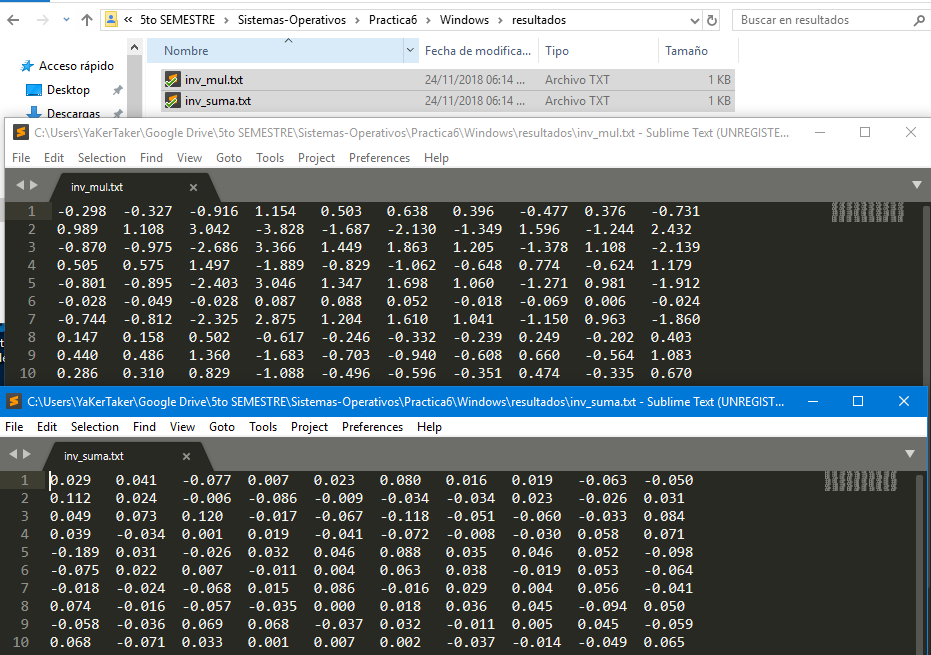
\includegraphics[width=0.87\textwidth]{Practica5/Images/windows/7_5.PNG}
			         \end{figure}
	                
	                 \begin{figure}[h!]
			          \centering 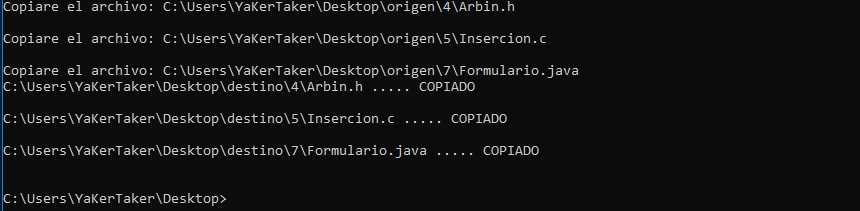
\includegraphics[width=0.87\textwidth]{Practica5/Images/windows/7_6.PNG}
			         \end{figure}
			         
			          \begin{figure}[h!]
			          \centering \includegraphics[width=0.72\textwidth]{Practica5/Images/windows/7_7.png}
			         \end{figure}
			         
			         \begin{figure}[h!]
			          \centering \includegraphics[width=0.72\textwidth]{Practica5/Images/windows/7_8.png}
			         \end{figure}
			         
			          \begin{figure}[h!]
			          \centering \includegraphics[width=0.72\textwidth]{Practica5/Images/windows/7_9.png}
			         \end{figure}
			         
			         \begin{figure}[h!]
			          \centering \includegraphics[width=0.9\textwidth]{Practica5/Images/windows/7_10.png}
			         \end{figure}
			         
			          \begin{figure}[h!]
			          \centering \includegraphics[width=0.9\textwidth]{Practica5/Images/windows/7_11.PNG}
			         \end{figure}
			         
			         \begin{figure}[h!]
			          \centering \includegraphics[width=0.9\textwidth]{Practica5/Images/windows/7_12.PNG}
			         \end{figure}
			         
	\end{itemize}	
	


% //////////////////////////////////////////////////////////////////////////////////////////////////////////////
%                                                   OBSERVACIONES
% /////////////////////////////////////////////////////////////////////////////////////////////////////////////
\newpage
	\section{Observaciones}
        
        \begin{itemize}
            \item[\Checkmark] Para los programas desarrollados en Linux, se utiliza el siguiente comando para compilar:
            
            \textit{gcc nombre\_programa.c -lpthread -o nombre\_programa}
            
            \item[\Checkmark] Algunas aplicaciones deben compilarse con atributos extras en el comando GCC y lpthread. La instrucción para compilar éstas aplicaciones se encuentra al inicio de su respectivo código.
            
            \item[\Checkmark] En el punto 3 de Linux, el segundo código de ejemplo para la creación de hilos en este sistema operativo, al momento de compilar con el comando de arriba, aparece un warning respecto al cast a tipo de variable void que se le hace al resultado del hilo cuando se regresa al main. A pesar de esto, la ejecución del programa es la esperada, por lo que podemos ignorarlo.
            
            \item[\Checkmark] En el punto 6 de Linux, el programa nos pide que ingresemos una ruta en donde se escribirán los archivos con los resultados de las operaciones con matrices. Ésta ruta debe ser ingresada de forma completa, por ejemplo: 
            
            \textit{\textbackslash home\textbackslash usuario\textbackslash Escritorio\textbackslash resultados}
            
            Esto aplica de igual manera para la entrada de las rutas en el punto 7.
            
            \item[\Checkmark] En las versiones de Windows de estos mismos programas, no es necesario ingresar la ruta completa.
            
             \item[\Checkmark] En este mismo punto, para la medición del tiempo de ejecucion de la aplicación, se utilizaron los códigos de \textit{tiempo.h} y \textit{tiempo.c} de la práctica 4.
            
            \item[\Checkmark] Es importante que tanto el directorio en donde se escribirán los resultados de las operaciones con matrices en el punto 6 como el directorio de destino en el punto 7 no existan antes de la ejecución de ambos programas, ya que de existir, ambos programas retornarán un error y acabarán su ejecución.
            
            \item[\Checkmark] Análogo al punto anterior, es necesario que la ruta de origen en el punto 7 exista antes de ejecutar el código.
            
            \item[\Checkmark] Las rutas que se utilizan en los puntos 6 y 7 se aceptan como parámetros de entrada por medio de la línea de comandos
            
             \item[\Checkmark] En el punto 7, la versión de Linux acepta todo tipo de archivos para copiarlos, sin embargo, la versión de Linux tiene problemas con las imágenes, por lo que únicamente funciona con archivos que contienen texto.
             
              \item[\Checkmark] Mientras que en Linux se usaron las llamadas al sistema scandir(), stat() y la estructura dirp(), en Linux se utilizo las llamadas al sistema FindFirstFile(), FindNextFile(), y variables de tipo WIN32\_FIND\_DATA.
             
            
            
            
            
            
        \end{itemize}
        
        


% //////////////////////////////////////////////////////////////////////////////////////////////////////////////
%                                                  ANALISIS CRITICO
% /////////////////////////////////////////////////////////////////////////////////////////////////////////////
	
	\section{Análisis Crítico}
	 La diferencia de la creación de múltiples hilos en los sistemas operativos Windows y Linux, es notable por la sintaxis que existen en ambos:
	    \begin{itemize}
	        \item Linux : Utilizamos las funciones de la biblioteca \textbf{pthread}, y el tipo de variable pthread\_t.
	        \item Windows: Utilizamos las funciones para manejo de hilos contenidas en la biblioteca \textbf{windows.h}, y los tipos de variable DWORD y HANDLE. Además, la función para un hilo es de tipo DWORD WINAPI.
	    \end{itemize}
	   
	   La manera de manejar hilos en cada sistema operativo cambia en la sintaxis que se usa. En Linux se usa pthread\_create() y pthread\_join(), mientras que en Windows se usa CreateThread() por medio de un manejador del id de cada hilo utilizando una variable de tipo HANDLE; para esperar a que todos los hilos terminen, utilizamos el mismo comando para procesos: WaitForSingleObject() ó WaitForMultipleObjects() para multihilos.
	   
	   Al ejecutar el programa de las matrices, hicimos una comparativa de los tiempos en los que se realiza teniendo los siguientes resultados:

    	\begin{figure}[h!]
    	    \centering
    	    \includegraphics[width=0.66\textwidth]{Practica5/Images/tiempos.PNG}
    	\end{figure}
        En el sistema operativo Windows, el usar hilos disminuye el tiempo respecto a la implementación secuencial y con creación de procesos, sin embargo en Linux no pasa eso, al contrario, el tiempo es exageradamente mayor con hilos que con procesos y en forma secuencial. 

% //////////////////////////////////////////////////////////////////////////////////////////////////////////////
%                                                   	CONCLUSIONES
% /////////////////////////////////////////////////////////////////////////////////////////////////////////////
	
	\section{Conclusiones}
	La programación multihilos sin duda tiene mucho campo de aplicación, desde los sistemas operativos hasta en la tecnologías que usamos cotidianamente.
	
	En la elaboración de este trabajo, después de discutir varios aspectos de la práctica nos dimos cuenta que obtuvimos conceptos que nos darán las bases para desarrollar aplicaciones en c en el sistema operativo tanto UNIX como Windows utilizando hilos, con la finalidad de poder realizar más de una tarea a la vez y administrando correctamente los recursos del equipo de cómputo.
	
	La utilidad de la programación con hilos resulta evidente. Por ejemplo, cualquier navegador web (FireFox, Chrome, Opera) puede descargar un archivo de un sitio o página web, y acceder a otro sitio al mismo tiempo. Si el navegador puede realizar simultáneamente dos tareas, no tendrá que esperar hasta que el archivo haya terminado de descargarse para poder navegar a otro sitio.
	
	En conclusión la programación multihilo esta presente en la mayor parte de las aplicaciones informáticas que usamos cotidianamente sin importar el lenguaje en que se desenvuelvan, el concepto de Thread o Hilo seguirá siendo el mismo

\end{document}